\documentclass[11pt, oneside]{article} 
\usepackage{geometry}
\geometry{letterpaper} 
\usepackage{graphicx}
	
\usepackage{amssymb}
\usepackage{amsmath}
\usepackage{parskip}
\usepackage{color}
\usepackage{hyperref}

\graphicspath{{/Users/telliott_admin/Tex/png/}}
% \begin{center} \includegraphics [scale=0.4] {gauss3.png} \end{center}

\title{Circular orbits}
\date{}

\begin{document}
\maketitle
\Large

\subsection*{Pythagoras and Newton}

A previous chapter looked in detail at Pythagoras' Theorem, which is used incessantly from here on out. Here, we explore one use of the Pythagorean theorem and provide a taste of orbital mechanics, which is a particular focus of calculus.  Newton made early calculations similar to these, which increased confidence about his famous inverse-square law and inspired the mathematics that led to the explanation of elliptical orbits.

Although the orbits of the planets around the sun are ellipses, they are very nearly circular and we will make that approximation for what follows here.

We use the Pythagorean Theorem to make another approximation.  Using $r$ for the (fixed) radius of the orbit for the moment, because the construction has capital letters for the points, including the symbol $R$:

\begin{center} 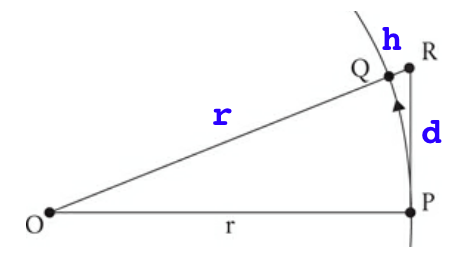
\includegraphics [scale=0.5] {pyth_circle1.png} \end{center} 

\[ r^2 + d^2 = (r + h)^2 = r^2 + 2rh + h^2 \]
\[ d^2 = 2rh + h^2 \]

If $h << r$ then we can ignore the very small quantity $h^2$ and obtain
\[ d^2 = 2rh \]
\[ r = \frac{d^2}{2h}, \ \ \ \ h = \frac{d^2}{2r} \]

If the planet were not accelerated, then it would move from $P$ to $R$, a distance $d$, and this is equal to the velocity $\times$ time:
\[ d = vt \]

At this point, we use an idea from calculus.  \emph{For a small enough segment of the orbit}, this distance $PR$ is the same as the arc length $PQ$.

\begin{center} 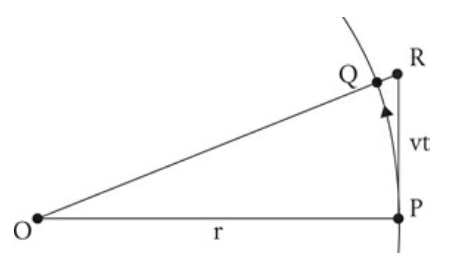
\includegraphics [scale=0.5] {pyth_circle2.png} \end{center} 

So we substitute for $d^2 = (vt)^2$ into the equation from above

\[ h = \frac{d^2}{2r} \approx \frac{(vt)^2}{2r} \]

\begin{center} 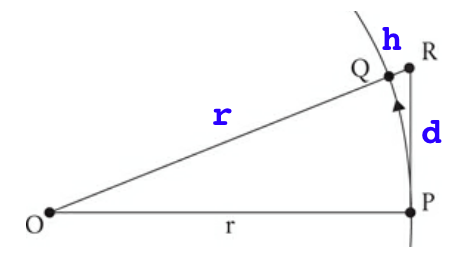
\includegraphics [scale=0.5] {pyth_circle1.png} \end{center} 

Also, for a small enough part of the orbit (again), $h$ and $d$ are perpendicular to each other as well.

At this point we use the additional assumption that the force is directed toward the sun.  We might say that the distance \emph{fallen} by the planet in this short time is $h$.  

By the standard equation of motion, under gravitational acceleration $g$ is related to $h$ and the time $t$ by this equation:

\[ h = \frac{1}{2} gt^2 \]

We combine the two different expressions for $h$

\[ h = \frac{1}{2} gt^2 \approx \frac{(vt)^2}{2r} \]
\[ g \approx \frac{v^2}{r} \]

Note:  we have not covered this yet.  If this idea (dependence on $t^2$) is completely new to you, you may want to come back to this part after going through the first \hyperref[sec:slopes]{\textbf{chapter}} on calculus.

The equation $a = v^2/r$ comes even more easily with a little bit of calculus and the use of vectors.  See \hyperref[sec:Uniform_circular_motion]{\textbf{here}}.

\subsection*{Kepler's Third Law}
The famous mathematician Johannes Kepler (of whom much more later also), working with observational data from Tycho Brahe, had the following values for the radius $R$ of the (assumed circular) orbit and the period $T$ (time for completion of one orbit), for five planets.

\begin{center} 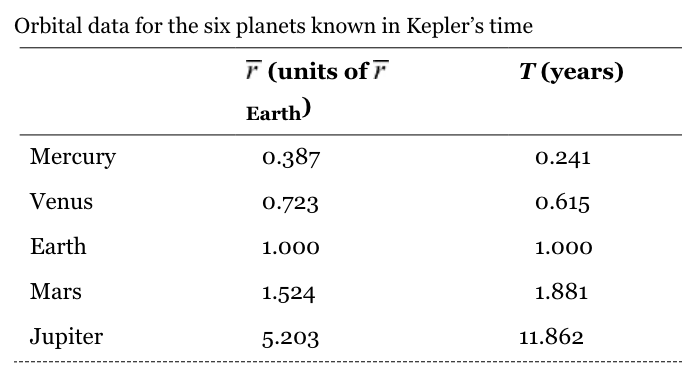
\includegraphics [scale=0.5] {K3_table.png} \end{center}
On the basis of this data, Kepler published his \textbf{third law} (in 1619, about $10$ years after the first two).  K3 states that
\[ T^2 = k R^3 \]

The square of the period is proportional to the cube of the radius of the orbit.  The data in the table has been scaled so that $k = 1$.

For a circular orbit, the orbital speed, the magnitude of the velocity $v = | \mathbf{v} |$, is constant. 

The period times the speed is equal to the circumference.  
\[ vT = C = 2 \pi R \]
\[ T = \frac{2 \pi R}{v} \]

K3 above says that
\[ R^3 = T^2 \]
\[ = \frac{(2 \pi)^2 R^2}{v^2}  \]
Hence
\[ v^2 \approx \frac{1}{R} \]
We showed above that the acceleration for a circular orbit is

\[ a = \frac{v^2}{R} = v^2 \cdot \frac{1}{R}  \]
so we conclude that that
\[ g = a \approx \frac{1}{R} \cdot \frac{1}{R} = \frac{1}{R^2}  \] 

if the acceleration of gravity $g$ is directed toward the sun, with a magnitude that is inversely proportional to the square of the distance, then we can explain Kepler's third law by running this chain of reasoning in reverse.

\subsection*{comparing the moon to an apple}
Earlier we worked out that the acceleration is
\[ a = \frac{v^2}{R} \]

Let's figure out the acceleration of the moon.  We make a decision to work in English units for this one.  

The moon averages about $237$ thousand miles from earth (221.5 - 252.7 thousand miles).  The earth's circumference is about $24.9$ thousand miles so its radius is about $3.96$ miles.  Thus, the ratio of the moon's distance to the center of the earth, compared to my distance to the center of the earth, is about $60:1$ (ranging between 56-64).

What is the moon's velocity?  The distance it travels in one complete orbit (in feet) is:
\[ 2 \pi \cdot 2.4 \times 10^5 \cdot 5280 \]
The time that takes in seconds is 
\[ 28 \cdot 24 \cdot 3600 \]
\[ v = \frac{2 \pi \cdot 2.4 \times 10^5 \cdot 5280}{28 \cdot 24 \cdot 3600} \]

The acceleration is $v^2/R$ so we square everything except the radius.
\[ a = \frac{(2 \pi)^2 \cdot 2.4 \times 10^5 \cdot 5280}{(28 \cdot 24 \cdot 3600)^2} = 0.0085 \]
That's in feet per second.

We compare this value to the acceleration measured at the surface of the earth, which is $32.2$ in the same units.  The ratio is $3788$, which is just over $(61.5)^2$.

Newton:

\begin{quote}I began to think of gravity extending to the orb of the Moon . . . and computed the force requisite to keep the Moon in her Orb with the force of gravity at the surface of the earth . . . \& found them answer pretty nearly. All this was in the two plague years of 1665-1666. For in those days I was in the prime of my age for invention \& minded mathematicks and Philosophy more than at any time since.\end{quote}

\end{document}